\documentclass[11pt]{article}
\usepackage[margin=1in]{geometry}
\usepackage{amsmath,amssymb}
\usepackage{booktabs}
\usepackage{graphicx}
\usepackage{hyperref}
\usepackage{xcolor}
\usepackage{natbib}

\graphicspath{{../results/}{../results/stack/}}

\newcommand{\todo}[1]{\textcolor{red}{[TODO: #1]}}
\newcommand{\gain}{\mathrm{gain}}
\newcommand{\ncd}{\mathrm{NCD}}
\newcommand{\pms}{\mathrm{PM}}

\title{Mechanism-Matched Data Scoring:\\
Compression Predicts and Accelerates the Formation of Induction Heads}

\author{Luca Columbu}
\date{Draft v0.4 --- \today}

\begin{document}
\maketitle

\begin{abstract}
Data selection for language-model pretraining is driven by scalars that
blend every capability together: loss under a reference model, similarity to
a target distribution, or redundancy. We propose scoring data against a
specific \emph{mechanism}: reverse-engineer the circuit a model must build,
reimplement its computation as a cheap program, and grade each document by
how much it exercises that program. We instantiate the principle for
induction heads, whose operation---locate the previous occurrence of the
current context and copy what followed---is the operation of the LZ77
compressor. On synthetic induction tasks, per-document compression gain
predicts the training step at which induction heads form
(Spearman $\rho=-0.98$, three seeds, two architectures), tracks the realised
copy length of the data at $\rho=0.995$ where the generating parameter
tracks it at $0.60$, and selects a training subset that matches a
copy-length oracle exactly. Mechanism tracing shows why: the copy-length
distribution selects among \emph{variants} of the induction circuit that
differ in attention lag, each with a fixed accuracy ceiling, so plateaus
previously read as partial learning are completed circuits of a
data-selected variant. A second compressor quantity, normalised compression
distance between documents, dissociates from gain and relates to
generalisation across name pairs rather than to formation. On real Python
code from The Stack, selecting a training subset by gain under a diversity
constraint makes induction heads form 1.5--2$\times$ sooner in attention and
2--3$\times$ sooner in behaviour than a random subset (three seeds, no
overlap), at a stable cost of 0.2 nats of validation loss that doubling the
budget does not remove; once formed, both circuits copy rare identifiers
equally well in distribution. The compressor's own match-length histogram
predicts, before training, on which corpora selection can act. The complete
real-data study cost under ten dollars of compute.
\end{abstract}

% ======================================================================
\section{Introduction}
% ======================================================================

The data that trains a language model is chosen by heuristics that
optimise a single quantity. Perplexity filters keep documents a reference
model finds neither too easy nor too hard~\citep{wenzek2020ccnet};
importance resampling matches a target
distribution~\citep{xie2023dsir}; domain reweighting learns a mixture from
a proxy model~\citep{xie2023doremi}; learnability-based selection keeps
points that reduce held-out loss~\citep{mindermann2022rho}; deduplication
removes near-copies~\citep{lee2022dedup,abbas2023semdedup,tirumala2023d4}.
These methods treat the model as a black box. They report averages over
benchmarks, and they cannot say which capability a given decision buys or
sells, because they never look at what the model builds.

Mechanistic interpretability has meanwhile produced detailed accounts of
individual circuits---induction heads~\citep{olsson2022induction},
indirect-object identification~\citep{wang2022ioi}, modular
arithmetic~\citep{nanda2023grokking}---and has shown that specific
distributional properties of training data switch some of them on and
off~\citep{chan2022data,reddy2023mechanistic}. That work varies the data
\emph{generator} and observes the model. It does not provide a way to grade
an arbitrary corpus before training.

This paper connects the two. The proposal is simple: \textbf{for a circuit
the model should build, find the cheapest algorithm that performs the same
computation, run it on each document, and use its output as a data score.}
We call this \emph{mechanism-matched scoring}, and we instantiate it once,
completely, for induction heads. The induction head's operation---find the
earlier occurrence of the current token, attend there, copy what
followed---is the operation of the LZ77 compression
algorithm~\citep{ziv1977lz77}, whose match statistics are exposed by any
\texttt{gzip} implementation. The use of compressors to estimate entropy and
cross-entropy of strings was developed
by~\citet{benedetto2002language,baronchelli2005zippers}; we use their two
quantities---per-document compression gain and cross-document compression
distance---and show that they measure two distinct properties of training
data with two distinct consequences for the trained model.

\paragraph{Contributions.}
\begin{enumerate}
\item \textbf{Compression gain predicts induction-head formation}
  (\S\ref{sec:gain}). Across repeat fractions, three seeds and two
  architectures, the formation step is a monotone function of gain
  ($\rho=-0.98$ attention-only, $-0.92$ with MLPs; $-1.0$ on condition
  means). Formation follows the score where the score and the repeated
  fraction disagree, and gain fails only where the token distribution
  changes.
\item \textbf{The compressor measures the causal variable better than the
  generator} (\S\ref{sec:oracle}). Gain tracks realised copy length at
  $\rho=0.995$; the repeat-fraction parameter that generated the data
  tracks it at $0.60$. Selection by gain matches a copy-length oracle
  (97\% subset overlap, identical formation) and beats selection by the
  generating parameter in three of three pools.
\item \textbf{Copy-length distribution selects the circuit variant}
  (\S\ref{sec:lag}). With MLPs present the induction circuit that forms
  keys on the token $k$ positions back; $k$ is set by the geometry of
  copies in the data, agrees across seeds, and fixes an exact accuracy
  ceiling. Plateaus at 0.66--0.76 are completed lag-$k$ circuits. We trace
  the lag to a positional copier the model builds before any induction head
  exists.
\item \textbf{Compression distance dissociates from gain and relates to
  generalisation, not formation} (\S\ref{sec:diversity}). The two
  quantities decorrelate across data knobs (pooled $r=-0.27$); with gain
  fixed, distance predicts generalisation across held-out name pairs
  (partial $+0.46$), gain predicts it negatively, and neither predicts when
  the task circuit forms. Generalisation to held-out roles is governed by a
  second circuit that in-document repetition trains.
\item \textbf{A learned scorer repairs the compressor's blind spot}
  (\S\ref{sec:tiers}). Where accidental matches swamp gain (small
  vocabularies), a reference model with an induction head restores
  prediction ($\rho$ from $-0.72$ to $-0.93$ pooled).
\item \textbf{On real code, selection accelerates formation at a measured
  cost} (\S\ref{sec:stack}). On 2.5B tokens of Python, a gain-plus-diversity
  subset forms induction heads 1.5--2$\times$ sooner in attention and
  2--3$\times$ sooner in behaviour than a random subset, pays 0.2 nats of
  validation loss stably across budgets, and yields an equally load-bearing
  copy head in distribution. The match-length histogram predicts in advance
  where selection can act: on children's stories it cannot, and does not.
\end{enumerate}

A methodological thread runs through the paper. Every synthetic task was
mechanism-traced \emph{before} it was swept, and this was not optional: the
first task we designed to elicit copying was solved by exclusion
(\S\ref{sec:twoname}), and the induction task was redesigned three times as
tracing exposed positional and fixed-offset shortcuts
(Appendix~\ref{app:redesign}). A data-selection claim that skips this step
is a claim about a mechanism the model may not have built.

% ======================================================================
\section{Related Work}
% ======================================================================

\paragraph{Data selection.}
Model-based scores---perplexity~\citep{wenzek2020ccnet}, learnability
\citep{mindermann2022rho}, gradient norms~\citep{paul2021el2n}---and
distribution-based scores---DSIR~\citep{xie2023dsir},
DoReMi~\citep{xie2023doremi}---optimise a global quantity.
Deduplication~\citep{lee2022dedup} and its semantic
variants~\citep{abbas2023semdedup,tirumala2023d4} remove redundancy and
report gains in average loss. Skill-It~\citep{chen2023skillit} orders data
by contribution to evaluation-defined skills. We differ in defining the
target as a circuit and the scorer as a reimplementation of that circuit's
computation, and in reporting circuit-level consequences that averages
hide.

\paragraph{Compression and language models.}
\citet{deletang2023compression} show that language-model loss is a
compression rate under arithmetic coding; \citet{huang2024compression}
report that compression rate correlates with downstream performance as a
global signal; \citet{jiang2023gzip} classify text with gzip distance. We
use compression as a circuit-specific detector and identify the internal
statistic---LZ77 match length---that carries the signal.

\paragraph{Induction heads and training data.}
\citet{olsson2022induction} identify induction heads and their abrupt
formation; \citet{chan2022data} show that burstiness, Zipfian skew and
class count in the data gate in-context learning; \citet{reddy2023mechanistic}
give a mechanistic model of the dynamics. Those works vary the generator
and observe the model. We measure the documents.

% ======================================================================
\section{Method}\label{sec:method}
% ======================================================================

\subsection{Compressor quantities}
Following \citet{baronchelli2005zippers}, the LZ77 code rate of a string
estimates its entropy, and compressing $B$ after $A$ estimates the
cross-entropy $C(A|B)\simeq(L_{A+B}-L_A)/L_B$, where $L_X$ is the
compressed length of $X$. We derive two quantities.

\emph{Gain.} Per-document compressibility beyond unigram statistics,
$\gain(B)=1-L_B/L_{\mathrm{shuf}(B)}$, where $\mathrm{shuf}(B)$ is a random
token permutation of $B$ (frequencies preserved) and $L$ is the zlib code
length in bits. Gain is large when a document contains long verbatim
repeats and zero for a document with no structure beyond its token
frequencies; single-token repeats and skewed unigram distributions do not
count.

\emph{Distance.} The normalised compression distance
$\ncd(A,B)=(L_{AB}-\min(L_A,L_B))/\max(L_A,L_B)$~\citep{li2004ncd}.
Corpus diversity is the mean $\ncd$ over a random sample of document pairs
at fixed length.

\emph{Match-length histogram.} LZ77 emits a sequence of (offset, length)
matches. The distribution of match lengths is the mechanistically
meaningful statistic underlying gain, and we use it as a pre-training
diagnostic of whether a corpus contains structure the score can act on. We
report the share of tokens covered by matches of length $\geq8$ and the
mean longest match per document.

All quantities are computed on token-id sequences with a sliding-window
LZ77 (zlib), reusing one compressor state for the context when computing
conditional scores.

\subsection{Why LZ77 matches induction}
An induction head~\citep{olsson2022induction} composes a previous-token
head, which writes ``preceded by $x$'' at each position, with a head that at
the current token $x$ attends to positions so labelled and copies the token
found there. LZ77 at each position searches backward for the longest string
that begins here and has already occurred, and emits a pointer to it. Both
locate the previous occurrence of the current context and reuse its
continuation. The compressor's match length is the length of the repeat
the induction head can exploit.

\subsection{Selection}
Given a pool of documents and a token budget, the \emph{gain} selector
ranks by gain and takes the top of the ranking. The \emph{gain + diversity}
selector proceeds greedily through the ranking, accepting a candidate only
if its $\ncd$ to each of 16 probe documents drawn from the already-accepted
set is at least 0.75, which rejects near-duplicates. We compare against
uniform random selection, against a half-gain, half-random \emph{mix}, and,
on synthetic data, against oracles that see the generating parameters.

% ======================================================================
\section{Synthetic Experiments}\label{sec:synth}
% ======================================================================

\subsection{Tasks}
\paragraph{Induction.} Random token sequences of length 64 over a
vocabulary of 100 tokens, containing a verbatim repeat of a random earlier
span at a random offset; the target inside the repeat is the token that
followed the earlier occurrence. The copy length is drawn uniformly up to a
maximum $\ell_{\max}$ set by the repeat fraction (16--31 across the sweep).
Knobs: repeat fraction, vocabulary, noise, number of copies at fixed
repeated fraction, and the copy-length distribution (uniform, fixed,
geometric, short-tailed). Appendix~\ref{app:redesign} records two earlier
versions that tracing showed to be solvable without content matching.

\paragraph{Two-name.} Template sentences with two names, one duplicated;
the target is the non-duplicated name, after~\citet{wang2022ioi}. Knobs:
pool size (4--64), Zipf skew (0--2), repetition rate (0--1), noise. Held-out
splits: names never used as the answer (held-out IO), name pairs never
co-occurring (held-out pairs), and a leak fraction in which held-out names
appear as answers. Generalisation is measured on single-sentence probes,
because the document-level metric is inflated by in-context repeats.

\subsection{Models and measurement}
Two-layer four-head transformers ($d_{\mathrm{model}}=128$) with rotary
positions by default; attention-only and with-MLP variants; 3L8H and 4L8H
replications. AdamW, learning rate $10^{-3}$, warmup 500 steps, no weight
decay unless stated. Three seeds per condition; checkpoints every 100
steps.

\emph{Formation step.} We use three definitions and report their
agreement: (i) behavioural, the first checkpoint at which validation
accuracy on copied tokens reaches 0.5; (ii) attention-based, the first
checkpoint at which any head places mass $\geq0.5$ on the token to be
copied at any lag (\S\ref{sec:lag}); (iii) patching-based, the first
checkpoint at which patching the layer-1 heads at target positions recovers
$\geq50\%$ of the clean-minus-corrupt logit difference under source-segment
corruption, with a 1-nat floor on the effect. Over 39 formed induction runs
(i) and (ii) agree at $\rho=+0.99$ with a mean gap of 87 steps, one
checkpoint interval; over 45 formed runs (iii) agrees with each at
$\rho=+0.96$, and final recovery is 0.97--1.00 everywhere. In attention-only
models patching and behaviour coincide (mean gap 70 steps); in MLP models
the patched circuit reaches 50\% recovery 1,000--2,000 steps before accuracy
reaches 0.5, the mechanistic form of the slower ``seep'' in those models.
Correlations below use the behavioural step unless stated.

\emph{Circuit analysis.} Per checkpoint and per head: attention mass to
the relevant positions and direct logit attribution, decomposed exactly
into heads, MLPs, embeddings and the LayerNorm-plus-unembed term.
Sharpness is the size of the greedy minimal sufficient head set that
restores 90\% of the logit difference with everything else mean-ablated per
position; faithfulness is accuracy with everything outside that set
ablated.

\subsection{Gain predicts formation}\label{sec:gain}

\begin{figure}[t]\centering
\includegraphics[width=0.48\textwidth]{zipper_vs_formation.png}\hfill
\includegraphics[width=0.48\textwidth]{zipper_vs_formation_mlp.png}
\caption{Formation step of the induction head against per-document gain.
Attention-only (left): $\rho=-0.98$ over 12 formed runs. With MLPs (right):
$\rho=-0.92$ over 18 formed runs. $\rho=-1.0$ on condition means in both.
Formation is a jump from accuracy $<0.2$ to $>0.8$ within one or two
100-step intervals; seed spread 0--200 steps.}
\label{fig:gain}
\end{figure}

Table~\ref{tab:gain} lists the repeat-fraction sweep. Below a gain of about
0.07 (attention-only) or 0.10 (MLPs) the circuit does not form within
budget. With MLPs, formation is two to four times later throughout and only
the densest condition snaps cleanly; the others plateau
(\S\ref{sec:lag}). Weight decay at $10^{-3}$ and $10^{-2}$ leaves
formation, lag and ceiling unchanged. A 3L8H attention-only replication
gives $\rho=-0.94$ over 9 formed runs (formation 2,600 / 1,300 / 933 for
repeat fractions 0.5 / 0.75 / 0.98) with the jumps intact.

\begin{table}[t]\centering\small
\begin{tabular}{lrrr}\toprule
Repeat fraction & Gain & Formation, attn-only & Formation, MLP \\\midrule
0.98 & 0.201 & 800   & 1,267 \\
0.90 & 0.181 & n/r   & 4,000 \\
0.85 & 0.175 & n/r   & 4,133 \\
0.75 & 0.154 & 900   & 4,367 \\
0.60 & 0.121 & n/r   & 5,467 \\
0.50 & 0.101 & 1,733 & 6,867 \\
0.35 & 0.068 & 3,600 & never ($>12$k) \\
0.20 & 0.034 & never ($>6$k) & n/r \\
0.10 & 0.012 & never ($>6$k) & n/r \\\bottomrule
\end{tabular}
\caption{Formation step (mean of three seeds) by condition; n/r, not run
in that sweep. Seed standard deviations are 0--200 steps (attention-only)
and 58--351 steps (MLP).}
\label{tab:gain}
\end{table}

Two further sweeps separate the score from the repeated fraction. Adding
noise lowers gain and delays formation together ($\rho=-0.92$). Splitting
a fixed repeated fraction into 1, 2 or 4 shorter copies lowers gain
(0.154, 0.149, 0.125) and delays formation (900, 1,267, 1,367;
$\rho=-0.88$): formation follows the score, not the fraction. The one
failure is the token distribution: at vocabulary 16 versus 100, gain
collapses (0.021 versus 0.101) while formation barely moves (1,367 versus
1,733), the wrong sign. \S\ref{sec:tiers} repairs this.

\subsection{The compressor measures copy length; the generator does not}
\label{sec:oracle}

In Table~\ref{tab:gain} gain is a deterministic function of the generating
parameter, so \S\ref{sec:gain} shows only that the compressor orders
repetition correctly. A selection experiment separates the two. From a pool
of 60,000 documents whose per-document repeat fraction is drawn from
$U(0.1, 0.98)$ and hidden, we select 20,000 by (a) gain, (b) the hidden
generating parameter, (c) realised copy length measured after generation,
(d) loss gain under a fixed reference model (\S\ref{sec:tiers}), and (e)
uniformly at random, and train three seeds on each.

Across three independent pools, gain-selected models form the circuit at
step 700 in every seed; reference-loss-selected at 700; parameter-selected
at 800--1,000; random at 5,200--6,000 or never within budget. The
copy-length-selected subset overlaps the gain-selected one by 97\% and
forms at step 700 in all three seeds with final accuracy 0.94--0.95, the
compressor's numbers exactly. The generating parameter is the worse
selector because it describes what was requested rather than produced: the
parameter sets a maximum copy length and the realised length is drawn below
it, so it tracks realised copy length at $\rho=0.60$ and admits documents
with high nominal repetition but short copies (24\% of its subset has copies
under 8 tokens; the compressor's has none). Gain tracks realised copy length
at $\rho=0.995$. All formed models have lag-0 circuits (attention mass
0.82--0.87). \todo{Figure: formation curves for the five arms.}

\subsection{Copy-length distribution selects the circuit variant}
\label{sec:lag}

\begin{figure}[t]\centering
\todo{lag figure: lag and ceiling against copy-length distribution}
\caption{With MLPs the induction circuit keys on the token $k$ positions
back (lag $k$). Holding $\ell_{\max}=24$: fixed-length copies give $k=0$,
formation at 800, accuracy 0.997; uniform lengths give $k=19$ and a 0.68
ceiling; geometric lengths give $k=22$--23, formation at 4,200--4,600 and a
0.59--0.62 ceiling; mostly-short copies never form. All three seeds agree
on $k$ in every condition.}
\label{fig:lag}
\end{figure}

A lag-$k$ induction circuit is a layer-0 head carrying the token $k+1$
positions back and a layer-1 head that matches the current token against
it and reads the token $k$ positions after the needed one. It copies
correctly whenever the copy offset exceeds $k$, so its accuracy ceiling is
the fraction of targets whose offset exceeds $k$. The ceiling is observed:
on targets with offset above the lag every model scores 0.88--0.93, on
targets with offset at or below it 0.01--0.07, and predicted and measured
ceilings agree (0.76 / 0.71 at lag 19, 0.83 / 0.73 at lag 12, 0.98 / 0.90
at lag 9--10).

Every MLP model in our sweeps built a lagged variant, with the lag agreeing
across seeds in every condition. Across the repeat-fraction sweep the lag
was 12, 15, 19, 21 and 22 for $\ell_{\max}$ of 16, 19, 24, 27 and 28, but
the lag follows neither the maximum nor coverage: at fixed
$\ell_{\max}=24$ it ranges from 0 to 23 depending only on the copy-length
distribution (Figure~\ref{fig:lag}). Attention-only models choose lag 0 at
every moderate repeat fraction and lag 8--9 at repeat 0.98 and at
vocabulary 16; MLP models never choose lag 0 except on fixed-length data.
Weight decay does not alter the lag.

\paragraph{Where the lag comes from.}
Relative-offset profiles across checkpoints show that before any induction
head exists, the MLP model builds a \emph{positional copier}: heads that
attend a fixed $d$ tokens back regardless of content, correct exactly when
the copy offset is $d+1$. The seed sits at the mode of the copy-offset
distribution (offset 24 in every dataset here, where accuracy spikes to
0.2--0.5 at offsets 22--25 and is near zero elsewhere at pre-formation
checkpoints). The induction head then grows on the seed and inherits its
offset: in every run the final lag equals the seed offset minus one, after
a drift of one or two positions during formation (uniform: seed 22, lag 19;
geometric: seed 23--24, lag 22--23). Fixed-length data yields the textbook
lag-0 circuit because its seed lives in layer 1 (all four layer-1 heads at
23 back from step 300) while layer 0 builds previous-token heads; the
broader distributions, with less mass at the mode (6--10\% of targets
against 21\%), seed layer 0 instead. So the lag is set by the geometry of
where copies sit relative to their sources, not by how much is copied. Two
corpora with identical gain but different source-to-copy offset
distributions produce different circuits. What decides the seed's layer is
the one untraced step.

Two consequences follow. The plateaus at 0.66--0.76 are not partial
circuits but complete lag-$k$ circuits whose ceiling is predicted by $k$; a
behaviour-only study would misreport them. And the variable that selects
the variant is the variable the compressor measures, which is why
\S\ref{sec:oracle} came out as it did.

\subsection{Compression distance dissociates from gain and relates to
generalisation, not formation}
\label{sec:diversity}

\begin{figure}[t]\centering
\includegraphics[width=0.9\textwidth]{diversity_pooled.png}
\caption{Gain and $\ncd$ across the three two-name knobs (45 runs), and
each outcome against each quantity.}
\label{fig:div}
\end{figure}

On the two-name task, repetition rate raises gain (0.10 to 0.34) with
$\ncd$ flat (0.67--0.73), and Zipf skew lowers $\ncd$ (0.728 to 0.647) with
gain flat (0.215--0.236); pooled with the pool-size sweep the two correlate
at $r=-0.27$. Table~\ref{tab:div} gives partial Spearman correlations on
single-sentence probes at the final checkpoint.

\begin{table}[t]\centering\small
\begin{tabular}{lrr}\toprule
Outcome & $\ncd$ (partial) & Gain (partial) \\\midrule
Formation, attention-based & $-0.04$ & $+0.03$ \\
Formation, patching-based  & $+0.16$ & $\phantom{+}0.00$ \\
Held-out pairs, accuracy   & $+0.46$ & $-0.19$ \\
Held-out pairs, logit difference & $+0.44$ & $-0.37$ \\
Held-out IO, accuracy      & $+0.19$ & $-0.21$ \\
Held-out IO, logit difference & $+0.06$ & $-0.07$ \\\bottomrule
\end{tabular}
\caption{Partial Spearman correlations over 45 two-name runs, each
compressor quantity controlling for the other. Diversity relates modestly
to generalisation across name pairs and gain negatively; neither predicts
formation of the exclusion circuit or generalisation to held-out roles.}
\label{tab:div}
\end{table}

Generalisation to held-out roles is governed instead by the repetition
rate of training documents, non-monotonically: probe accuracy on held-out
IO names is 0.00, 0.25, 0.40, 0.06, 0.05 at rates 0, 0.25, 0.5, 0.75, 1.
In-document repetition trains a content-independent copy mechanism whose
promotion of in-context names extends to the held-out ones and counteracts
the prior of \S\ref{sec:twoname}, until at high repetition the copy shortcut
replaces the task circuit altogether. This is an interaction between the
two circuits of this paper, observed on mixed data.

Formation is flat across every knob except the extremes. At pool size 4
the task is memorised; at repetition rate 1.0 every later sentence repeats
an earlier one, an induction shortcut pre-empts the task circuit, and
formation is delayed from 333 to 1,500 steps: the regime in which data
admits a cheaper mechanism and the model builds that instead of the
target.

\subsection{The two-name circuit is exclusion, not copying}
\label{sec:twoname}

The task was designed to elicit name-copying after~\citet{wang2022ioi}. The
model built something else. Two layer-1 heads attend to the duplicated
name with mass 0.94--0.99 and push its logit down; no head places more than
0.2 attention on the answer. The answer's margin of 10--12 logits over
pool names absent from the prompt comes from MLP~1 and MLP~0 fed by
layer-0 attention, not from a name-mover. Patching the two heads recovers
86--100\% of the logit difference; ablating them collapses held-out-IO
accuracy to zero in every run and validation accuracy to 0.43--0.51 in five
of twelve, a third head serving as backup in the rest. Greedy sufficient
sets are 2--5 of 8 heads in 2L4H models (one S-inhibition head plus one or
two layer-0 heads) and 7--9 of 32 in a 4L8H replication, spread over three
layers with several backup S-heads.

\paragraph{Priors and their cost.}
Names never used as answers acquire a prior against being the answer,
carried by MLP~0 (the unembed-bias term is $<0.1$ everywhere). The prior
forms \emph{during} circuit formation---the held-out logit difference
deepens to about $-4.5$ over the first 250 leaked examples---then climbs
linearly at about 0.01 logits per leaked example and crosses zero after
600--1,000 examples, roughly 1\% of sentences seen; a leaked example costs
about 800 examples' worth of erosion before formation and 100 after. Zipf
skew weakens the prior faster than it costs pair generalisation (held-out
IO 0.36 to 0.63 at the document level; crossing 2,600 to 267 steps).

\subsection{A learned scorer repairs the compressor's blind spot}
\label{sec:tiers}

\begin{figure}[t]\centering
\includegraphics[width=0.9\textwidth]{tiers_vs_formation.png}
\caption{Formation step against the compressor score (left) and against
the reference-model score (right), 39 induction runs in four families. The
two agree except in the vocabulary family, where the compressor's score
collapses and the model's does not.}
\label{fig:tiers}
\end{figure}

At vocabulary 16, accidental short matches compress the shuffled baseline
as well as the document, and gain collapses (0.021 versus 0.101 at
vocabulary 100) while formation does not. A fixed reference model with an
induction head, scoring each dataset by its loss gain over shuffled
documents, rates vocabularies 16, 32 and 100 at 0.090, 0.099 and 0.104
where gain says 0.021, 0.038 and 0.101. Pooled over 39 induction runs,
Spearman with formation is $-0.72$ for gain and $-0.93$ for the reference
model; the entire gap is the vocabulary family, and within every other
family the two agree (Figure~\ref{fig:tiers}). Gain and the model's loss
are the same quantity under two compressors~\citep{deletang2023compression};
the learned one wins exactly where LZ77's matching is uninformative. The
learned scorer depends on its reference having the circuit: in
\S\ref{sec:oracle} it matched gain document for document only because its
reference was the one random-arm seed that had formed.

% ======================================================================
\section{Real Corpora}\label{sec:real}
% ======================================================================

\subsection{Children's stories: the diagnostic predicts a null}
\label{sec:tinystories}

On a 65M-token slice of TinyStories no induction head forms in any of seven
runs; the prefix-matching score never leaves its initialisation baseline.
The match-length histogram says why: median LZ77 match of 2 tokens,
0.1--0.35\% of tokens in matches of $\geq8$, against 27\% in the synthetic
subset that forms at step 700. Selection moves bigram repeats from 12\% to
18\% and long matches by tenths of a percent. Natural-prose induction rides
on single-token repeats (47\% of tokens), which the shuffled-baseline gain
discounts, and reported prose phase changes sit at $10^9$--$10^{10}$
tokens~\citep{olsson2022induction}, 15--150 times this budget. The score
has no range here and the model has no budget here; the histogram
identified the first before any model was trained.

\subsection{Python code: selection accelerates formation}
\label{sec:stack}

\paragraph{Setup.}
The Python split of the deduplicated Stack~\citep{kocetkov2022stack},
streamed to 2.5B tokens under a word-level vocabulary of 32,768 tokens
(8.1\% unknown-token share) and cut into 9.77M windows of 256 tokens.
Of the pool's tokens, 26\% sit in LZ77 matches of $\geq8$ (mean longest
match 28), against 27\% in the synthetic subset of \S\ref{sec:oracle}; in
the gain-ranked top fifth the share is 62\% (mean longest 61), and in the
diversity-constrained selection 57\% (50). Arms: gain-plus-diversity
selection (greedy by gain, $\ncd\geq0.75$ to 16 probes; 247k of the 2.2M
windows scanned rejected) and uniform random selection, 1.95M windows
each. Model: 4 layers, 8 heads, $d_{\mathrm{model}}=256$, rotary
positions, batch 64, learning rate $10^{-3}$, warmup 500, bf16; 30,000
steps (491M tokens, one pass over the arm), three seeds each, checkpoints
every 500--1,000 steps; one seed per arm continued to 60,000 steps (983M
tokens, a second pass). Measures: the prefix-matching score
of~\citet{olsson2022induction} (best head, top-512 tokens) and induction
accuracy on repeated random sequences the model has not seen; validation
loss on 20,000 held-out windows; and an in-context delta on rare
identifiers (below).

A preliminary local experiment on 64M tokens of installed-package Python,
repeated over epochs, grew a head five times stronger in the selected arm
but formed in neither; fresh data at the same budget, not more steps, was
the fix, as with TinyStories (Appendix~\ref{app:local}).

\paragraph{Formation.}
\begin{table}[t]\centering\small
\begin{tabular}{llrrrrr}\toprule
Arm & Seed & $\pms\geq0.5$ & Ind.\ acc $\geq0.5$ & Final $\pms$ & Final ind.\ acc & Val loss \\\midrule
Gain + div. & 0 & 1,000 & 2,000 & 0.75 & 0.86 & 1.80 \\
Gain + div. & 1 & 1,000 & 2,000 & 0.89 & 0.86 & 1.80 \\
Gain + div. & 2 & 1,000 & 2,000 & 0.83 & 0.84 & 1.78 \\
Random      & 0 & 2,000 & 6,000 & 0.82 & 0.70 & 1.60 \\
Random      & 1 & 1,500 & 4,000 & 0.74 & 0.78 & 1.61 \\
Random      & 2 & 2,000 & 5,000 & 0.74 & 0.73 & 1.59 \\\midrule
Gain + div., 983M & 0 & 1,000 & 2,000 & 0.75 & 0.86 & 1.745 \\
Random, 983M      & 0 & 2,000 & 5,500 & 0.84 & 0.70 & 1.557 \\\bottomrule
\end{tabular}
\caption{The Stack, 491M tokens unless stated. Formation steps are the
first checkpoint at which the measure reaches 0.5; seed 0 has checkpoints
every 1,000 steps, seeds 1--2 every 500.}
\label{tab:stack}
\end{table}

\begin{figure}[t]\centering
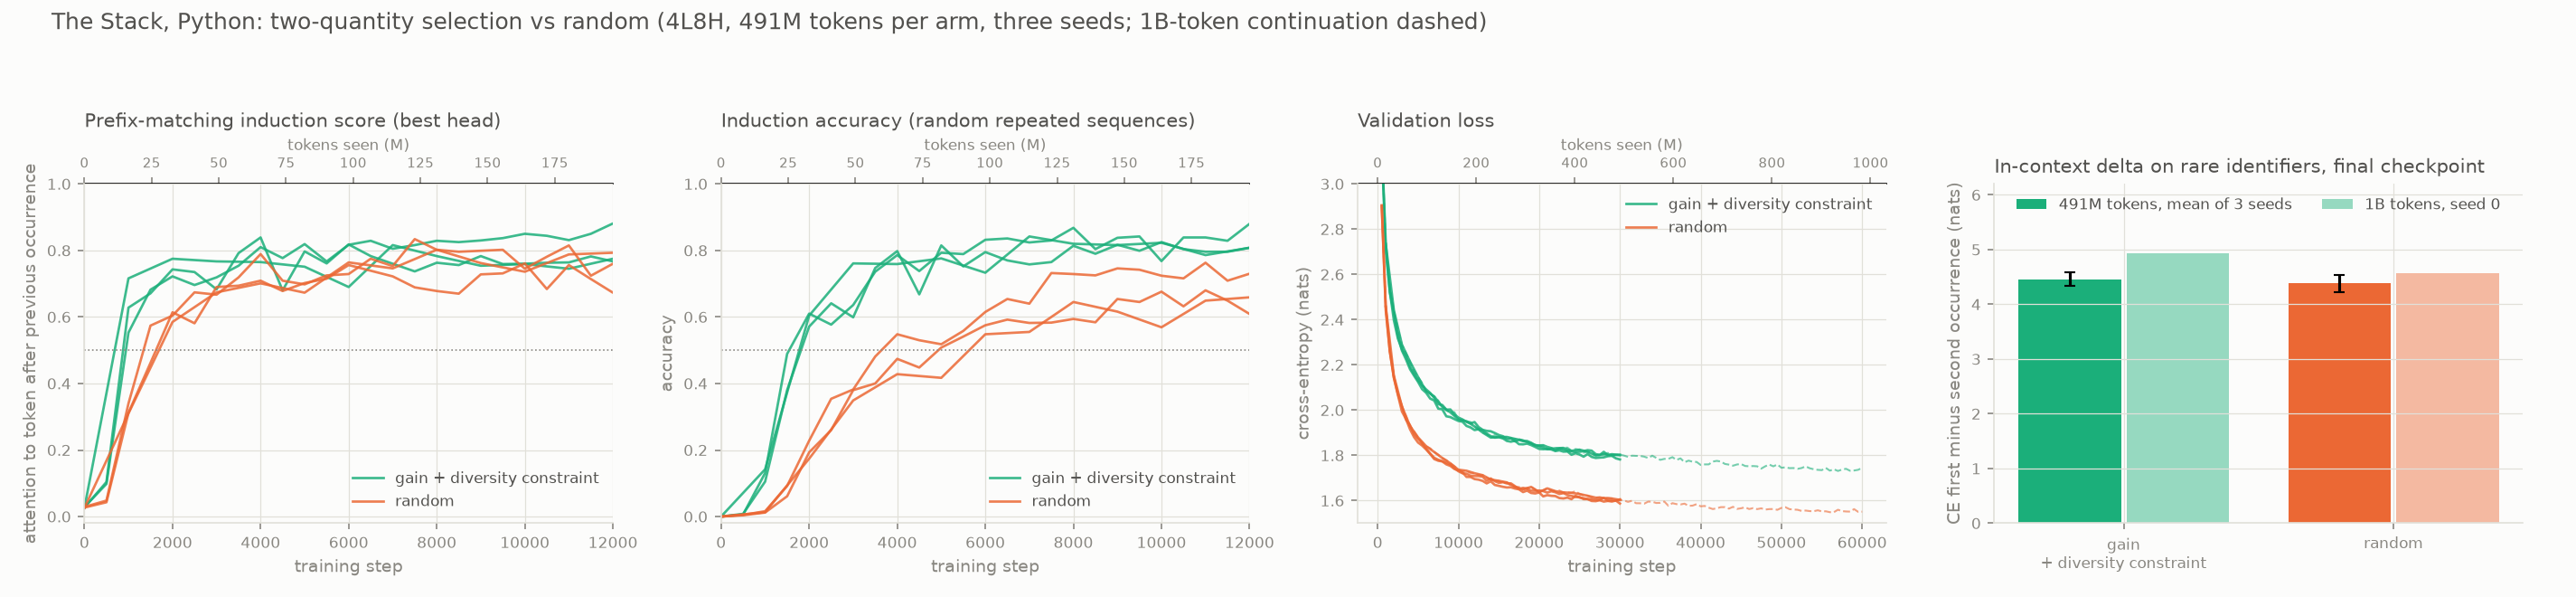
\includegraphics[width=\textwidth]{stack_trajectories.png}
\caption{The Stack. Prefix-matching score and induction accuracy over the
formation window for both arms and three seeds; validation loss to 983M
tokens (dashed: the continued seed); the in-context delta on rare
identifiers at the final checkpoint. The selected arm snaps
(prefix-matching 0.10 to 0.55--0.72 between steps 500 and 1,000; induction
accuracy 0.38--0.49 to 0.57--0.61 between 1,500 and 2,000); the random arm
seeps (prefix-matching 0.31 to 0.46--0.61 over steps 1,000--2,000; induction
accuracy 0.17--0.23 at 2,000, 0.43--0.55 at 4,000, 0.55--0.62 at 6,000).}
\label{fig:stack}
\end{figure}

The selected arm forms the head at step 1,000 in every seed and the
behaviour at step 2,000 in every seed; the random arm at 1,500--2,000 and
4,000--6,000 (Table~\ref{tab:stack}): 1.5--2$\times$ sooner in attention and
2--3$\times$ sooner in behaviour, with no overlap on either measure. The
selected arm's induction accuracy stays 0.06--0.16 above the random arm's
to the end of training while prefix-matching overlaps (0.75--0.89 versus
0.74--0.84): both heads attend where they should, and the selected model
executes the copy more accurately on random sequences. Doubling the budget
leaves formation and final induction accuracy unchanged in both arms and
improves validation loss by 0.05 in both; the 0.2-nat gap between arms
persists and the loss curves never cross. The trajectories reproduce,
between two selections of one real corpus, the snap-versus-seep contrast
observed between the attention-only and MLP models of
\S\ref{sec:gain} (Figure~\ref{fig:stack}).

\paragraph{In-context delta.}
Absolute loss on repeated identifiers orders like validation loss and so
measures distribution quality, not the head. We instead measure, for each
rare identifier (not among the 2,000 most frequent names in a 1M-window
sample) occurring at least twice in a validation window, the cross-entropy
at its first occurrence $\mathrm{CE}_1$ and at its second $\mathrm{CE}_2$;
the delta $\mathrm{CE}_1-\mathrm{CE}_2$ is the in-context benefit, and
distribution quality cancels. As controls we compute the same delta for
repeated common tokens and a name-swap test in which the identifier is
replaced throughout the window's prefix by a substitute name, reporting the
loss moved off the original name, the loss moved onto the substitute, and
how often the model then prefers the substitute.

\begin{table}[t]\centering\small
\begin{tabular}{llrrrrr}\toprule
Arm & Seed & $\mathrm{CE}_1$ & $\mathrm{CE}_2$ & Delta (frac.\ $>0$) & Common-token delta & Prefers swap \\\midrule
Gain + div. & 0 & 9.14 & 4.56 & 4.58 (0.86) & 0.74 & 0.57 \\
Gain + div. & 1 & 9.06 & 4.78 & 4.28 (0.84) & 0.73 & 0.57 \\
Gain + div. & 2 & 9.07 & 4.54 & 4.53 (0.86) & 0.73 & 0.58 \\
Random      & 0 & 8.39 & 3.98 & 4.41 (0.88) & 0.66 & 0.54 \\
Random      & 1 & 8.20 & 4.02 & 4.18 (0.87) & 0.66 & 0.47 \\
Random      & 2 & 8.29 & 3.73 & 4.56 (0.88) & 0.66 & 0.54 \\\midrule
Gain + div., 983M & 0 & 9.20 & 4.27 & 4.93 (0.86) & 0.72 & 0.60 \\
Random, 983M      & 0 & 8.16 & 3.59 & 4.56 (0.88) & 0.66 & 0.55 \\\bottomrule
\end{tabular}
\caption{In-context delta on 4,807 rare-identifier pairs and 20,867
repeated-common-token pairs from 2,000 validation windows, final
checkpoints. Delta declines with occurrence distance in every arm alike
(5.1--5.5 nats at $\leq32$ tokens; 2.7--3.0 at 128--256).}
\label{tab:delta}
\end{table}

The copy head is load-bearing in distribution in both arms: 4.2--4.9 nats
on rare identifiers, positive for 84--88\% of them, six times the delta on
common tokens, and the swap control moves 5--6 nats off the original name
and 7.4--8.9 onto the substitute, with the model preferring the substitute
about half the time. At the end of training the two arms copy about
equally (mean delta 4.46 versus 4.38 over three seeds, within seed spread);
$\mathrm{CE}_1$ orders like validation loss, the distribution cost again.
At 983M tokens the selected arm's delta is 4.93 versus 4.56, a modest edge
on one seed.

\paragraph{Reading.}
On real code, selection by the compressor buys \emph{when} the induction
circuit forms and a circuit that copies more accurately on syntax-free
sequences; it does not buy in-distribution copying once both circuits
exist, and it costs 0.2 nats on the distribution that doubling the budget
does not recover. The synthetic finding transfers---gain governs formation
and a gain-heavy selection pays on the distribution---and the
recommendation is unchanged: use both compressor quantities.

\paragraph{Trade-off curve at small scale.}
On the local 64M-token pool, four arms at matched size---gain only, gain
plus diversity, half gain and half random, random---order monotonically on
validation loss (2.43, 2.30, 2.13, 2.03) and on the loss at repeated rare
identifiers (6.20, 5.68, 5.13, 4.74), while the diversity-constrained arm
grows the strongest head of any (prefix-matching 0.10--0.12 in two seeds
versus 0.03--0.07 for gain only), and the mix keeps a head twice random's.
Rejecting near-duplicates removes cross-document repetition, which an
in-context copy head cannot use, and keeps within-document repetition,
which it can. The trade-off is tunable, and the two quantities set its two
axes (Figure~\ref{fig:fourarms}). \todo{repeat the four arms on The Stack
if budget allows.}

\begin{figure}[t]\centering
\includegraphics[width=\textwidth]{phase3_code_four_arms.png}
\caption{Local Python pool, four arms, three seeds, 8,000 steps:
prefix-matching by checkpoint, validation loss, and loss on repeated
low-frequency identifiers at the final checkpoint.}
\label{fig:fourarms}
\end{figure}

% ======================================================================
\section{Discussion}\label{sec:discussion}
% ======================================================================

\paragraph{The principle.}
Gzip predicts induction not because compression measures data quality in
general but because LZ77 and the induction head perform the same
computation. The generalisation is not ``use gzip'' but ``for each circuit,
find the cheapest program that computes what the circuit computes.'' Where
no such program is at hand, a small model that has already learned the
circuit is a learned implementation of it (\S\ref{sec:tiers}).

\paragraph{What averages hide.}
Deduplication lowers gain; our results predict, and \S\ref{sec:stack}
shows the converse of, a delay in induction. Outlier filtering lowers
diversity; \S\ref{sec:diversity} predicts a cost in generalisation across
rare combinations. Neither cost appears in a loss average.
Mechanism-matched scores make them measurable before training, and the
match-length histogram says on which corpora a given score can act at
all.

\paragraph{Data picks the variant.}
That the copy-offset geometry sets a circuit parameter with a built-in
ceiling (\S\ref{sec:lag}), that in-document repetition trains a second
circuit whose reach over held-out names rises and then collapses
(\S\ref{sec:diversity}), and that two selections of one real corpus yield
circuits that copy equally in distribution but unequally on syntax-free
sequences (\S\ref{sec:stack}), suggest a broader question: which data
statistics set which circuit parameters. We have one traced law and one
real-data echo of it.

\paragraph{Limitations.}
Models of 2--4 layers; one circuit family; one learning rate. The
real-data acceleration is measured at formation steps of one to six
thousand, early relative to any production budget; the persistent
difference is in the circuit's generality, not its in-distribution use.
The lag mechanism is traced to the positional seed but the choice of the
seed's layer is not explained. The exclusion circuit's formation is
insensitive to every data property varied, so the two-name task tests
generalisation, not formation. Prose corpora at our budget are below the
induction phase change, and our diagnostic correctly reports that the
score has no range there, but we have not shown selection acting on prose.
The 0.2-nat distribution gap is a fixed cost of selecting a fifth of a pool
by any compression criterion and would need a mix or a curriculum to
remove.

\paragraph{Future work.}
A second circuit where the hand-written scorer should fail and the learned
one should win: synthetic facts with paraphrases, where gain selects
against the data that builds retrieval and $\ncd$ selects for it. What
decides the seed's layer. The four-arm trade-off on The Stack.
Interference between circuits on mixed data, of which the repetition-rate
result is a first instance.

\paragraph{Reproducibility.}
All synthetic experiments run on a laptop CPU or its integrated GPU. The
complete real-code study---data download, tokenisation, scoring, eight
training runs to 491M--983M tokens, and analysis---cost about \$6.60 of
rented GPU and CPU time plus a network volume. Code, findings log and this draft: \url{https://github.com/lucacolumbu/LLM-research}.

\bibliographystyle{plainnat}
\bibliography{refs}

\appendix
\section{Induction-task redesigns}\label{app:redesign}
Three versions were built; each was mechanism-traced before sweeping.
(1) Fixed repeat offset: solved by a layer-0 positional head with no content
matching. (2) Random offset, fixed length: content matching present, but
keyed on ``the token $r$ positions back'' because a fixed copy length
privileges that feature. (3) Random offset and length: no shortcut
remains; used throughout. Learned absolute positions with a short warmup,
not weight decay, were found to block formation in an early MLP
configuration; weight decay of 0, $10^{-3}$ and $10^{-2}$ gives identical
formation, lag and ceiling.

\section{Local code pool}\label{app:local}
12,037 installed-package Python files, 498k windows of 128 tokens; top
100k windows by gain versus three random 100k subsets; 2L4H, 8,000 and
24,000 steps. Gain of subset 0.365 versus 0.162; 45\% versus 14\% of tokens
in matches $\geq8$ (mean longest match 30 versus 13). Prefix-matching at
8,000 steps 0.03--0.07 (rising from step 5,000) versus 0.01 flat; at 24,000
steps 0.17 versus 0.03; validation loss 2.41 versus 1.90. In-context delta
on rare identifiers 1.7--2.0 nats in every arm, name-swap control
1.3--1.8 nats, with no ordering by arm: at this budget the accelerated head
was not yet load-bearing. Four-arm results in \S\ref{sec:stack}.

\section{Additional figures}
\begin{figure}[h]\centering
\includegraphics[width=0.7\textwidth]{leak_sample_efficiency.png}
\caption{Held-out IO accuracy against leaked examples seen, two-name task.}
\end{figure}
\todo{per-run patching summaries; tier comparison per family.}

\end{document}
